\documentclass[utf8, zavrsni]{fer}
\usepackage{graphicx}
\usepackage{booktabs}
\usepackage{hyperref}
\usepackage{algorithm}
\usepackage{algpseudocode}
\usepackage{listings}
\usepackage{subfig}
\graphicspath{{Images/}}

\begin{document}

\thesisnumber{6391}
\title{Detekcija i klasifikacija tekstovnih elemenata na slici koristeći duboke neuronske mreže}
\author{Lukas Šestić}
\maketitle

\zahvala{ Zahvaljujem se prof. dr. sc. Domagoju Jakoboviću na pruženoj pomoći i sredstvima danima u svrhu uspješne izrade završnog rada. 

Također se zahvaljujem svojim roditeljima na prilici za studiranje i stalnoj podršci.
}

\tableofcontents

\chapter{Uvod}
\section{Uvod}
Računalna moć uređaja koje gotovo neprestano nosimo sa sobom kao što su pametni telefoni i prijenosna računala je unazad deset godina eksponencijalno narasla. Naravno, sa modernim alatima dolaze i moderni problemi. 


Jedan najraširenijih alata, koji se sve više i više koristi za rješavanje problema koji su do nedavno bili nemogući, ili izrazito algoritamski komplicirani za riješiti je \emph{umjetna inteligencija}.
Umjetna inteligencija podrazumjeva skup načina i metoda koje računalu opisuju početno i konačno stanje do kojeg mora doći sam.


Ovaj rad, bavit će se najkorištenijom metodom umjetne inteligencije, \emph{dubokim učenjem}, i njegovim podskupom \emph{računalnim vidom}.
Kroz rad i programsku implementaciju, prihvatiti ću se problema detekcije napisanog teksta na slici i daljnom obradom istog. \\
Detaljno ću kroz poglavlja obraditi postupke koje sam primjenio za generiranje raznolikih slika koje imitiraju rukopis i proces potreban da računalo nauči prepoznavati isti na slici.


Na kraju, izlučeni tekst sa slike, biti će moguće obraditi na željeni način.
Način koji ću ja predstaviti biti će primjena jednostavne matematike, slično onome što pruža \emph{Photomath, Inc.}. 
Na primjer, za sliku na kojoj je napisan tekst \texttt{"2 + 2"}, izlaz će biti slika sa kvadratima oko prepoznatih simbola, i rješenje obrađenog teksta, u ovom slučaju \texttt{"4"}.

\section{Računalni vid}

\subsection{Pregled}
Na najvišoj razini, \emph{računalni vid} su metode koje koje računalima daju mogučnost razumjevanja slike na visokoj razini, najčešće s ciljem automatiziranja ljudskih poslova.
Osnovni zadatak je raspoznavanje veze između obrazaca na slici i rješenja na problem koji želi riješiti. Svi procesi koji koriste strojno učenje, u konačnici se svode na  detekciju i klasifikaciju elemenata na slici. Metode računalnog vida temelje se na geometriji, statistici, fizici i teoriji učenja. \\
Danas, se velika količina problema rješava uz pomoć računalnog vida, često da ljudi za to nisu ni svjesni:
\begin{itemize}
\item Prepoznavanje znakova (Slika ~\ref{fig:cv_traffic_1})	
\item Prepoznavanje lica
\item Kompresija i restauracija slike
\item Prepoznavanje elemenata na slici
\item Analiza medicinskih snimki u svrhu detaljnije analize
\item Itd.
\end{itemize} 

\begin{figure}[h!]
	\centering
	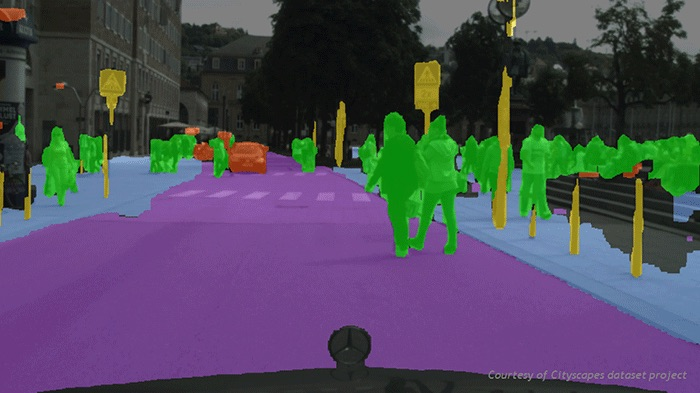
\includegraphics[width=0.8\linewidth]{cv_traffic}
	 \caption{Maskiranje elemenata na slici prometa}
 	 \label{fig:cv_traffic_1}
\end{figure}

\subsection{Konvolucijske neuronske mreže}
Konvolucijske neuronske mreže danas se koriste kao najefektivniji način postizanja računalnog vida. Glavna prednost nad potpuno povezanim neuronskim mrežama je manji broj \emph{težina} za treniranje što znatno ubrzava treniranje. Ipak, ono što je možda najvažnije za napomenuti je to što pozicija traženog elementa na slici \emph{konvolucijskoj neuronskoj mreži} ne igra ulogu. 

Svaki sloj \emph{duboke konvolucijske neuronske mreže} funkcionira kao filter koji se kreće po slici, pamteći što ga je najviše aktiviralo. Najčešće se koristi filter veličine \texttt{3 x 3}.
(Slika ~\ref{fig:conv_net_1})

Dalje, uz konvolucijski sloj, nerijetko se postavlja \emph{max pooling sloj}. Na apstraktnoj razini, princip rada max pooling sloja je sljedeći: Ako uzmemo veličinu pooling filtra kao onu koja se najčešće koristi, to jest \texttt{2 x 2}, on izlaz iz prethodnog sloja raspodjeli na kvadrate iste veličine. Zatim, filter se postavi između 4 kvadrata i sebi za vrijednost stavi najveću iz svakog u pripadajuće polje. \\ 
Prirodno je pitati se zašto se to koristi i zašto to radi. \\
Pooling filter jednostavno smanjuje "rezoluciju" prethodnog sloja, ne mjenjajući važne čimbenike potrebne za daljnji rad mreže. Na primjer, vertikalna linija, krug, ili elipsa, ostaje ono što je, jedino manje razlučivo. 
Bitno je napomenuti da smanjivanjem rezolucije dobivamo puno manje parametara za treniranje. 
Stavimo to u brojeve. Slike unutar \emph{mnist} seta podataka su veličine \texttt{28 * 28}. To znači da bi se treniralo $28*28$ parametara. Primjenom \emph{Max pooling sloja} veličine \texttt{2 x 2}, treniralo bi se $\frac{1}{4}*(28*28)$ parametara. 

\begin{figure}[h!]
	\centering
	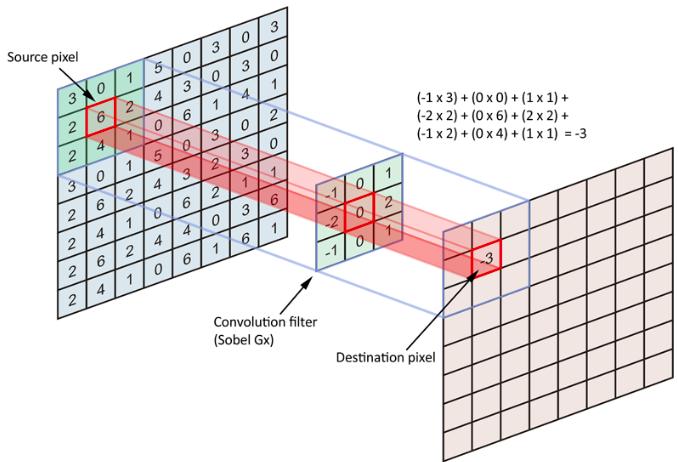
\includegraphics[width=0.5\linewidth]{conv_net}
	 \caption{Klizeći konvolucijski filter}
 	 \label{fig:conv_net_1}
\end{figure}

Spomenute prednosti, referenciraju se na glavnu značajku \emph{konvolucijskih mreža}. Cilj je ići dublje, ne šire. Za sliku veličine \texttt{100 x 100}, potpuno povezanoj neuronskoj mreži u prvom sloju treba \texttt{10 000} čvorova, svaki sa svojim parametrom za treniranje, dok konvolucijskoj to ne treba. \\
Svaki sljedeći sloj ima drugu ulogu. Prvi najčešće ima ulogu raspoznavanja najosnovnijih elemenata slike kao što su različiti rubovi, dok sve dublji koriste podatke od prošlih i osnovne elemente grupiraju u apstraktne strukture koji predstavljaju značajnije elemente slike.


\chapter{Generiranje skupa podataka}
\section{Značaj podataka u dubokom učenju}
Prvi i najdulji praktični korak treninga predstavlja priprema podataka. 
Sve ovisi o zadatku koji mreža mora riješiti, ali, generalno je pravilo da je više podataka bolje.
Konačna kvaliteta rješenja osim o arhitekturi mreže koju dizajniramo, ovisi o kvaliteti podataka kojom ju usmjeravamo.
Priprema podataka vrši se u 3 glavna koraka \cite{generalDatasets}:
\begin{enumerate}
\item Prikupljanje
\item Klasifikacija
\item Označavanje
\end{enumerate} 
\subsubsection{Prikupljanje podataka}
Prikupljanje podataka mora biti sustavan i smislen proces jer može otežati i olakšati daljnje korake. 
Najpreporučeniji način za prikupljanje je dugoročno i postepeno spremanje podataka jer rezultira velikim brojem objektivnih i kvalitetnih podataka.
Odlučeno je koristiti metodu računalnog generiranja vlastitog skupa podataka. 
Razlog tome je raznolikost elemenata koje mreža mora moći detektirati i fleksibilnost koju dobivamo jednom kada ustanovimo sve potrebe.
\subsubsection{Klasifikacija i označavanje podataka}
Generirani podaci na određeni način moraju biti prikazani mreži. 
Iako u mrežu slika ulazi kao vektor dimenzija \texttt{(visina x širina x kanali)}, mreži su potrebni i podaci za uspoređivanje rezultata i računanje uspješnosti.
U ovom radu koristi se \texttt{.csv} datoteka za dohvaćanje i kao opisnik slika. 
Postupak automatskog generiranja slika uvelike je olakšao klasifikaciju i označavanje jer je cijeli postupak ostvaren kao "cjevovod".
Pri izlasku, slika bi bila prikazana kao na slici ~\ref{fig:pipelineExitExample}.
Datoteka bi upisano imala ime slike, simbol na slici, širinu, visinu i točan položaj elementa na slici. 
Prednost ovog pristupa je i u tome što slika nije zadana apsolutnom putanjom, što znači da su slike mogle biti kreirane na vlastitom računalu, prenešene na udaljeni server za treniranje i bez komplikacija biti korištene. \\
Veličina opisnika je također bila zanemariva. \\ 
Nakon raspodjele \texttt{80:20} za trening i validaciju na 15 000 slika, veličine su bile \texttt{440kB} i \texttt{110kB} dok je direktorij sa slikama bio veličine \texttt{6,7GB}.

\begin{figure}[h!]
	\centering
	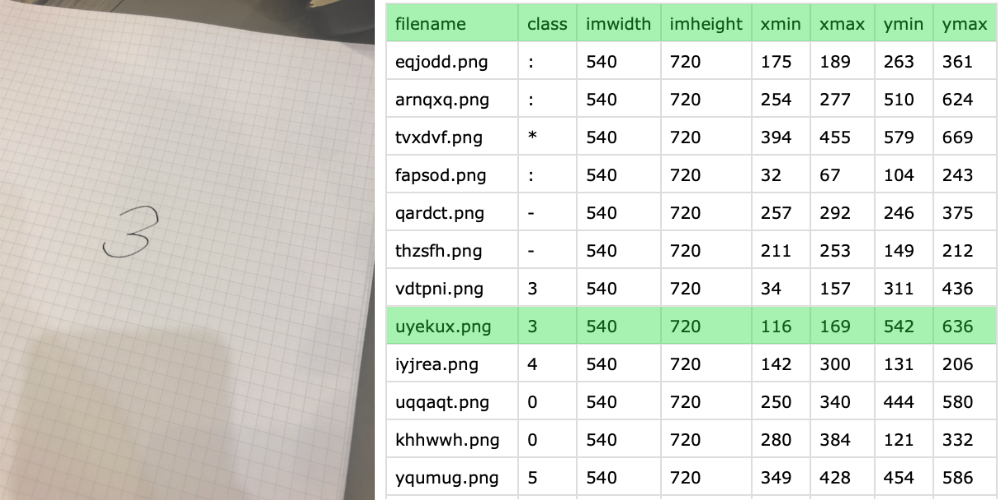
\includegraphics[width=1.0\linewidth]{image_csv}
	 \caption{Slika i pripadajuća referenca u .csv datoteci}
 	 \label{fig:pipelineExitExample}
\end{figure}

\section{Generiranje slika}
\subsection{Generalizacija postupka}
Za relativan uspjeh treniranja mreže za detekciju i klasifikaciju 14 tekstovnih elemenata (0-9, +, -, *, :) rezultati su pokazali da je potrebno minimalno 10 000 slika. 
Ne samo zbog broja elemenata već i zbog složenosti i raznolikosti između njih. 
Razvijeni postupak primjenjuje sve taktike \cite{chollet2017deep} potrebne za stvaranje raznovrsnog i kvalitetnog seta podataka.
Zbog transformacija opisanih u daljnjim dijelovima poglavlja, gotovo je nemoguće, da iako se isti font stavlja na pozadinu, nastane isti oblik.
Na slici ~\ref{fig:imageGenerationPipeline} prikazana je topologija cjevovoda koja kreira slike.
Cijeli cjevovod implementiran je unutar programskog paketa \emph{ImageGenerator}, razvijen u svrhu apstraktiranja cijelog postupka.
\begin{figure}[h!]
	\centering
	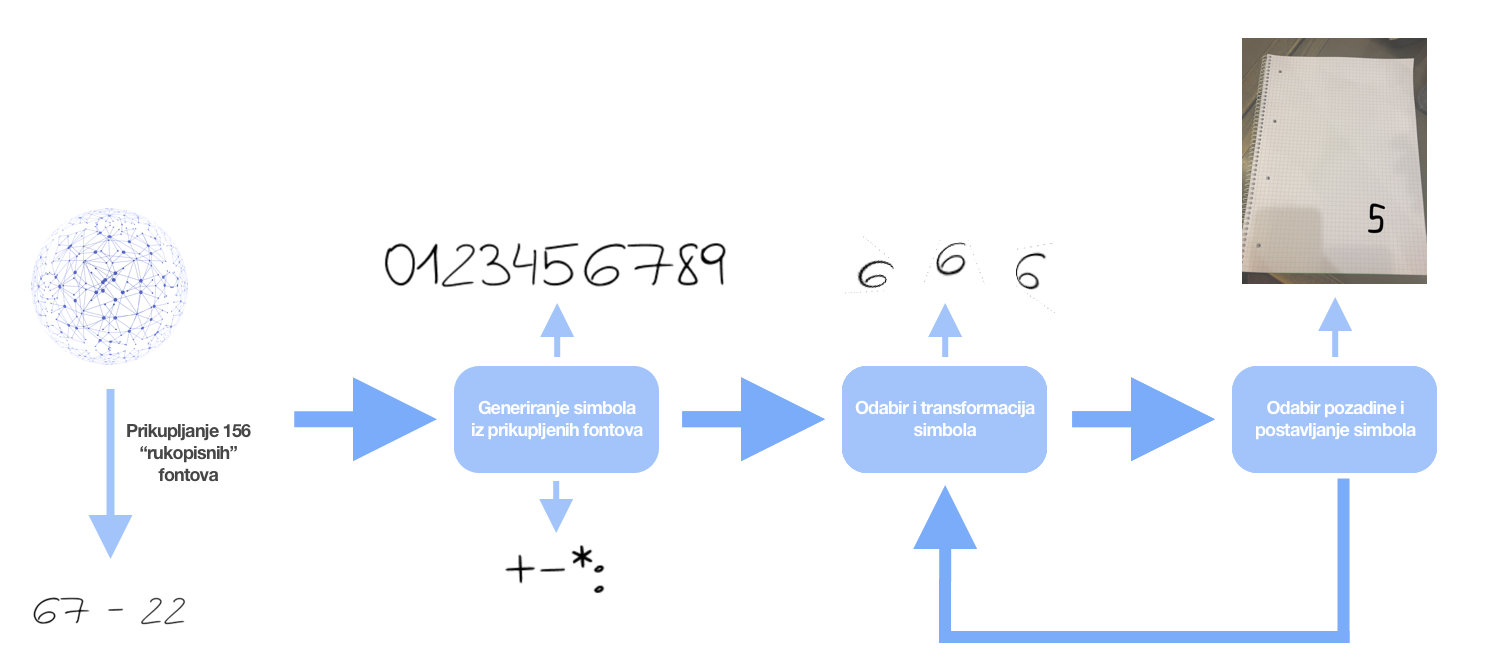
\includegraphics[width=1.0\linewidth]{image_generation_pipeline}
	 \caption{Prikaz visoke razine cjevovoda za generiranje slika}
 	 \label{fig:imageGenerationPipeline}
\end{figure}

\subsection{Prikupljanje fontova}
Ispisivanje velikog broja simbola sa razlikom između varijacija istog monoton je i neisplativ posao, posebice zbog dostupnosti svih potrebnih resursa na internetu.
U prilog je također išlo to što su dostupni fontovi, koji primjenjuju rukopisni stil, najčešće zbilja napisani rukom i vektorizirani, pa generiranje i transformiranje neće negativno utjecati na kvalitetu.
Osim rukopisnih fontova, prikupljen je i mali broj fontova koji su stilski između čistog rukopisnog i tipkanog. \\
Fontovi su bili prikupljeni sa sljedećih izvora, a na slici ~\ref{fig:fontDiffs} vidljivi su primjeri istih:
\begin{itemize}
\item \url{https://www.dafont.com}
\item \url{https://www.1001fonts.com}
\item \url{https://www.1001freefonts.com}
\end{itemize}
\begin{figure}[h!]
	\centering
	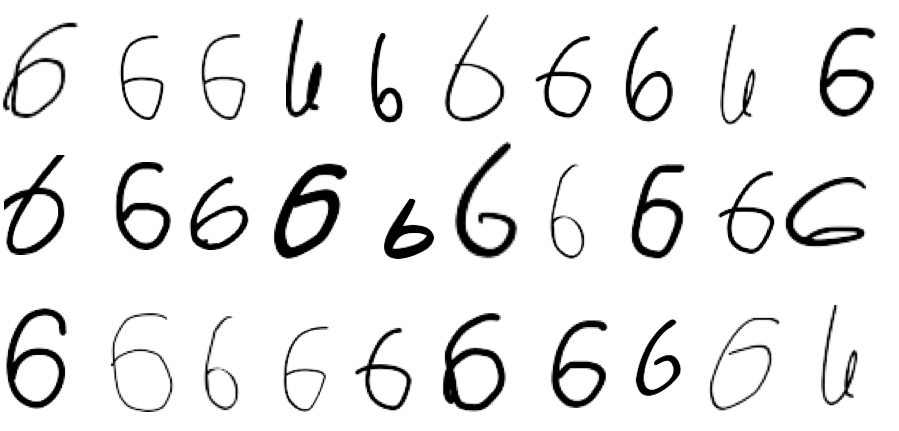
\includegraphics[width=0.85\linewidth]{font_diffs}
	 \caption{Varijacije unutar simbola uzrokovane fontovima}
 	 \label{fig:fontDiffs}
\end{figure}

\subsection{Generiranje simbola}
Nakon prikupljanja i sortiranja fontova, generiranje samih simbola bio je jednostavan posao.
Važno je očuvati transparentnost pozadine iza simbola jer u trenutku kada se postavi na pozadinu po izboru, ona mora biti vidljiva.
\begin{algorithm}
\caption{Generiraj sve simbole}
\begin{algorithmic}[1]
	\Function{generirajTextSliku}{$font, simbol$}
		\State $velicina \gets font.velicina(simbol)$
		\State $slika \gets Image('RGBA', velicina, (255, 255, 255, 0))$
		\State $slika.text = simbol$
		\State \Return $slika$
	\EndFunction
	\Function{generirajSveSimbole}{\null}
		\For{\texttt{simbol in simboli}}
			\For{\texttt{font in fontovi}}
				\State $direktorijSimbola \leftarrow spoji(putDoSimbola, simbol)$
				\If{$direktorijSimbola\ ne\ postoji$}
					\State \Call{kreirajDirektorij}{$direktorijSimbola$}
				\EndIf
				\State $generirana slika \gets$ \Call{generirajTextSliku}{$font, simbol$}
				\State \Call{spremiSliku}{$generiranaSlika$}
			\EndFor
		\EndFor
	\EndFunction
\end{algorithmic}
\end{algorithm}

\subsection{Transformacije}
Prije postavljanja simbola na nasumično odabranu sliku, svaki simbol prošao je kroz tri točke transformiranja:
\begin{enumerate}
\item Skaliranje
\item Rotacija
\item Afina transformacija
\end{enumerate}
Cilj transformacija je maksimalno unijeti raznolikost unutar skupa podataka u slučaju premalog ili presličnog broja slika.
Klasa \emph{ImageGenerator} za to se brine na sličan način kao programski paket \emph{Keras.preprocessing.image.ImageDataGenerator} \cite{Keras.io}.
Transformacije nad slikama izvedene su pomoću programskog paketa \emph{OpenCV} \cite{OpenCV} jer apstraktira potrebne matematičke operacije na razumljiv, lako koristiv i prilagodljiv način.
Tijekom faze transformiranja i postavljanja slike na pozadinu, one su u obliku matrice definirane pomoću programskog paketa \emph{Numpy}.
\subsubsection{Skaliranje}
Skaliranje pomoću \emph{OpenCV} paketa može se izvoditi ili ručno, specifirajući točnu veličinu, ili dajući faktor skaliranja.
\emph{OpenCV} također automatski primjenjuje \emph{interpolaciju} kako bi se kvaliteta maksimalno sačuvala.
Skaliranje se izvodi na način da se matrica slike pomnoži sa matricom skaliranja, zadanom na sljedeći način:
$$
M
=
\begin{bmatrix}
	s_{x} & 0 \\
	0 & s_{y}
\end{bmatrix},
$$
gdje je $s_{x}$ faktor skaliranja u $x$ dimenziji, a $s_{y}$ faktor skaliranja u $y$ dimenziji.
Rezultat skaliranja vidljiv je na slici ~\ref{fig:scaling}
\lstset{numbers=left}
\lstinputlisting[language=python]{CodeSamples/Scaling.py}
\begin{figure}[h!]
	\centering
	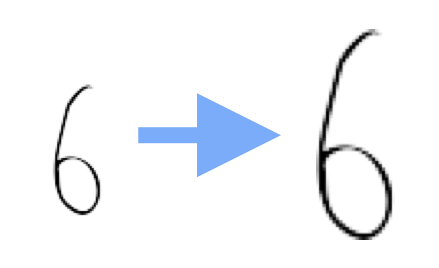
\includegraphics[width=0.4\linewidth]{Scaling}
	 \caption{Rezultat primjene skaliranja uz faktore $s_{x} = s_{y} = 1.25$}
 	 \label{fig:scaling}
\end{figure}
\subsubsection{Rotacija}
Rotacija slike za kut $\theta$ ostvaruje se množenjem s matricom rotacije:
$$
M
=
\begin{bmatrix}
	\cos(\theta) && -\sin(\theta) \\
	\sin(\theta) && \cos(\theta)
\end{bmatrix}
$$
Iako je rotiranje izvedeno iz središnje točke, \emph{OpenCV} nudi podršku za eksplicitno zadavanje točke oko koje će se rotacija izvoditi.
Rezultat rotiranja vidljiv je na slici ~\ref{fig:Rotating}.
\lstset{numbers=left}
\lstinputlisting[language=python]{CodeSamples/Rotation.py}
\begin{figure}[h!]
	\centering
	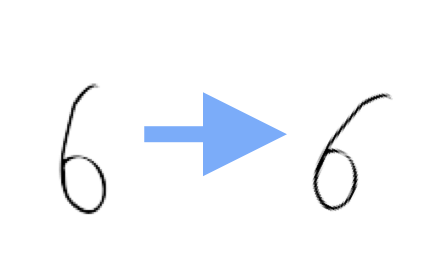
\includegraphics[width=0.4\linewidth]{Rotation}
	 \caption{Rezultat primjene rotacije s $\theta = 25$}
 	 \label{fig:Rotating}
\end{figure}
\subsubsection{Afine transfromacije}
Afine transformacije koristimo za prividno transformiranje simbola "u prostoru", bez velikog rizika od prevelike distorzije slike jer, sve paralelne linije nakon transformacije ostaju paralelne.
\emph{OpenCV} afinu transformaciju vrši tako da tri odabrane točke na slici pomakne za određeni koeficijent.
Kao i ostale transformacije, matematički nastaje množenjem matrice slike s matricom afine transformacije oblika:
$$
\begin{bmatrix}
	1 && \tan(\beta) \\
	\tan(\alpha) && 1
\end{bmatrix} ,
$$
gdje su $\alpha$ i $\beta$ razlike u kutevima prema pripadajućim koordinatnim osima.
Rezultat primjene afine transformacije na simbolu vidljiv je na slici ~\ref{fig:Affine}
\lstset{numbers=left}
\lstinputlisting[language=python]{CodeSamples/Affine.py}
\begin{figure}[h!]
	\centering
	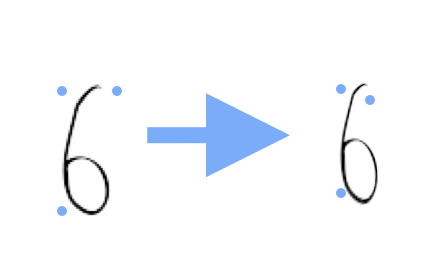
\includegraphics[width=0.4\linewidth]{Affine}
	 \caption{Rezultat primjene afine transformacije s pripadajućim referentnim točkama}
 	 \label{fig:Affine}
\end{figure}

\subsection{Kreiranje cjelovitih slika}
Kreiranje cjelovitih slika svodilo se na postavljanje generiranih i transformiranih simbola na pozadinu po izboru.
Pozadina također igra veliku ulogu u prepoznavanju jer mreža pregledava cijelu sliku.
Za potrebe ovog rada izabrana je pozadina matematičkih bilježnica uz pretpostavku da bi se iste najčešće koristile kada bi se naučena mreža koristila u stvarnom svijetu.
Izlazi iz mreže vidljivi su na slikama ~\ref{fig:ImageGeneratorOutputs} i ~\ref{fig:ImageGeneratorTermOutputs}.
Slike su spremljene u direktorij \texttt{Images}, a \texttt{.csv} opisnik u direktorij \texttt{Data} odakle će se dalje referencirati za kreiranje \texttt{.record} datoteke za daljnje korištenje \emph{Tensorflow-u}.
\begin{figure}
	\subfloat[Izlazna slika iz \emph{ImageGenerator-a}] {%
		
\includegraphics[width=0.4\linewidth]{image_generator_output} %
		\label{fig:ImageGeneratorOutputs}
	}

	\subfloat[Ispis za praćenje statusa generiranja slika] {%
		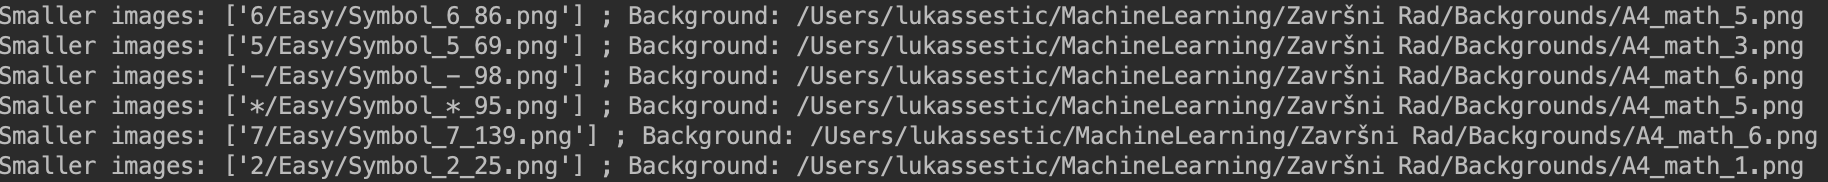
\includegraphics[width=1.0\linewidth]{image_generator_term_output} %
		\label{fig:ImageGeneratorTermOutputs}
	}
\end{figure}

\section{TFRecords}
Zašto je bolje za mrežu da podatke čita iz \texttt{.record} datoteke nego odvojeno slike i pripadajuće opise?
Zamislimo sljedeći scenarij.
Učenje se izvodi na računalu sa \texttt{HDD} diskom, slike i oznake su u različitim direktorijima.
Svako čitanje sljedeće slike i oznake rezultira potencijalnim pomicanjem glave diska.
Cilj je da sve potrebne datoteke budu što bolje poravnate u memoriji.
Tu se pokazuje najveći značaj \emph{TFRecords} datoteke. 
Jedna binarna datoteka koja sadrži sve informacije za mrežu, jedinstveno poravnata u memoriji \cite{TFRecords}. \\
U pozadini, \emph{TFRecords} je format koji koristi \emph{Protocol buffer} tehnologiju.
\emph{Protocol buffer} ili kraće \emph{Protobuf} je knjižnica za efikasnu serijalizaciju strukturiranih podataka (\cite{tensorflow.org}).
Konkretno, koristimo \emph{Protobuf} poruke oblika \texttt{"string" : value} za predstavljanje objekata mreži.
U mom slučaju, slike su zapisane na sljedeći način:
\begin{itemize}
\item height = \texttt{int64}
\item width = \texttt{int64}
\item filename = \texttt{bytes}
\item sourceid = \texttt{bytes}
\item encoded = \texttt{bytes}
\item format = \texttt{bytes}
\item xmins = \texttt{float\_list}
\item xmaxs = \texttt{float\_list}
\item ymins = \texttt{float\_list}
\item ymaxs = \texttt{float\_list}
\item classes\_text = \texttt{bytes\_list}
\item classes = \texttt{int64\_list}
\
\end{itemize}
Svi navedeni podaci zapisuju se pod ključ \texttt{feature}. \\
Kako u našem slučaju vršimo detekciju i klasifikaciju objekata, bitno je da na neki način i klasama damo jedinstveni identifikator.
Naime, u \emph{TFRecords} datoteku pod ključ \emph{classes} koji sadrži podatke o tom koji su svi objekti na slici ne pišemo doslovno ime objekta (npr. automobil, kuća, ...).
Pišemo brojčanu vrijednost istog objekta koja ga predstavlja. 
Isti način je precizniji i sažetiji. \\
Primjerice, ime dnevnika koji sadrži mapiranja iz objekta u njegovu brojčanu vrijednost naziva se \emph{Label map} i osim za stvaranje \emph{TFRecords} datoteke, koristi ga i sama mreža i mi kad iz mreže čitamo što je ista prepoznala.
Za kreiranje datoteke praćeni su koraci opisani na službenoj \emph{Tensorflow} stranici.


\chapter{Single Shot MultiBox Detector mreža}
\section{Zašto je nastala SSD mreža}
\emph{Single Shot MultiBox Detector} (dalje \emph{SSD}) je mreža za detekciju i klasifikaciju kojoj je primarna svrha jednostavnost i brzina.
Prije nastanka \emph{SSD} mreže, najpoznatije mreže za isti zadatak bile su implementirane arhitekturom \emph{Region-Convolutional Neural Network} (dalje \emph{R-CNN}).
\emph{R-CNN} mreže na izlazu tipično daju set kvadrata koje opisuju objekt i klasu istog.
Klasični izlaz iz \emph{R-CNN} mreže vidljiv je na slici ~\ref{fig:ObjectDetectionOutput}.
Osim bazičnog, iz \emph{R-CNN}-a nastale su i mreže \emph{Fast(er)-R-CNN} koje dalje ubrzavaju i poboljšavaju preciznost iste arhitekture (\cite{ren2015faster}).
No, nijedna od tih nije uspjela doseći gotovo "real-time" brzinu sa značajnom preciznosču
\begin{figure}[h!]
	\centering
	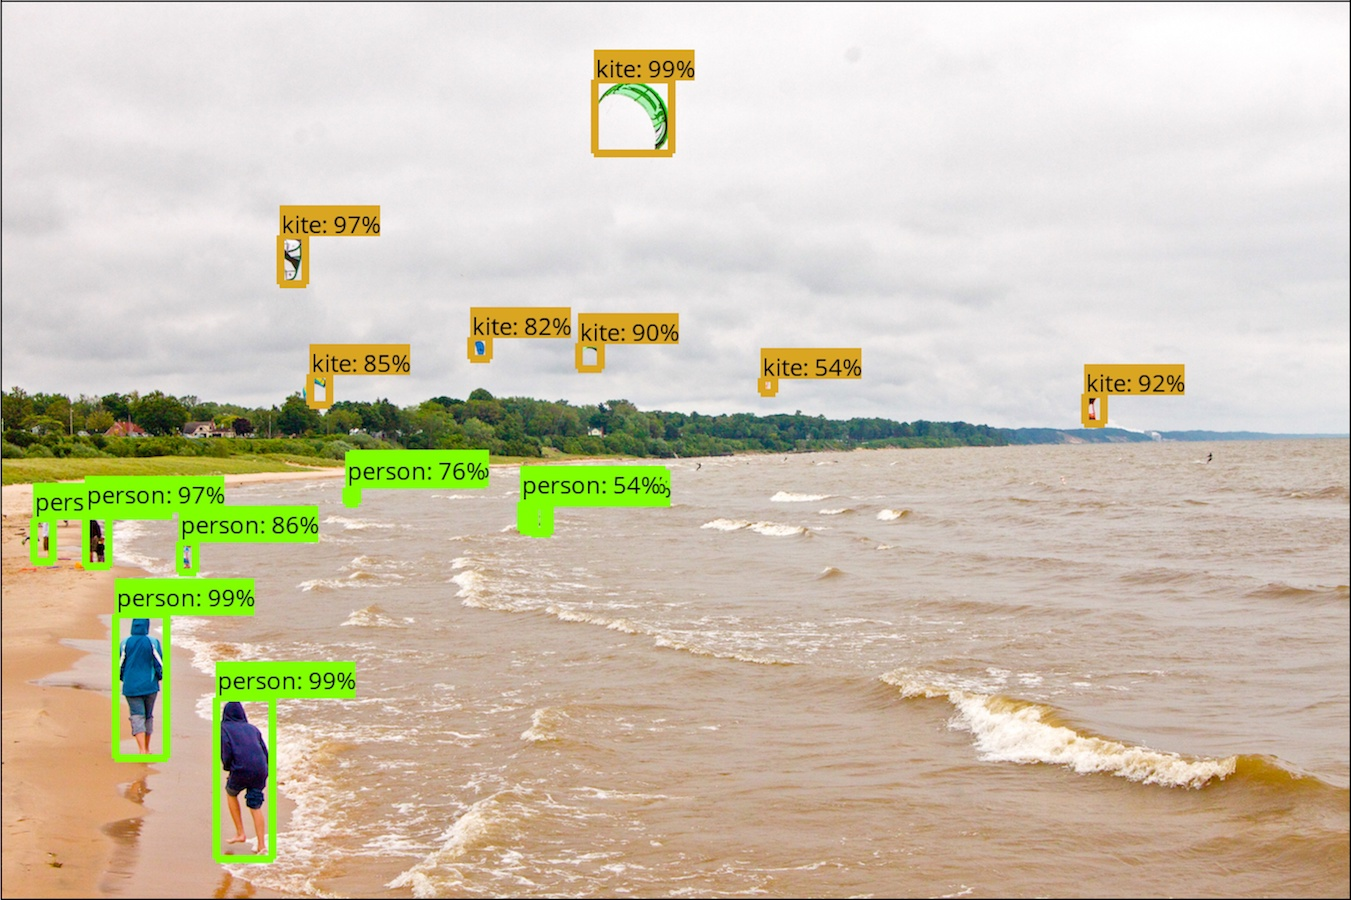
\includegraphics[width=1.0\linewidth]{object_detection_output}
	 \caption{Tipični izlaz iz mreže za detekciju i klasifikaciju sa prikazanim kvadratima i klasama}
 	 \label{fig:ObjectDetectionOutput}
\end{figure} \\
Iako su spomenute mreže imale pokazivale impresivne rezultate, također su imale i nekolicinu problema:
\begin{itemize}
\item Više faza treniranja
\item Komplicirana mreža
\item Mreža spora za stvarno korištenje
\end{itemize}
Zbog spomenutih problema, nastale su nove arhitekture od kojih je jedna i \emph{SSD}, koju ovaj rad koristi cjelokupnu implementaciju zadatka detekcije i klasifikacije 14 različitih klasa.

\section{Arhitektura}
\subsection{VGG-16 arhitektura}
\emph{VGG-16} je poznata neuronska mreža nastala na Oxfordu od strane \emph{Visual Geometry Group}-a, odakle i potječe ime.
Mreža sama po sebi ostvaruje odlične rezultate na \emph{ImageNet} datasetu no to nije jedini razlog zašto je jedna od najkorištenijih. \\
\emph{VGG} mreža razvijena je da bude jednostavna, sadržavajući samo \texttt{3x3} konvolucijske i \texttt{2x2} pooling slojeve prije završnih gusto spojenih slojeva (\cite{simonyan2014very}).
Arhitektura mreže vidljiva je na slici ~\ref{fig:VGGArchitecture}
Također, cijela struktura, težine i cijela istrenirana mreža je dostupna besplatno na internetu na službenoj stranici projekta (\url{http://www.robots.ox.ac.uk/~vgg/research/very_deep/}).
\begin{figure}[h!]
	\centering
	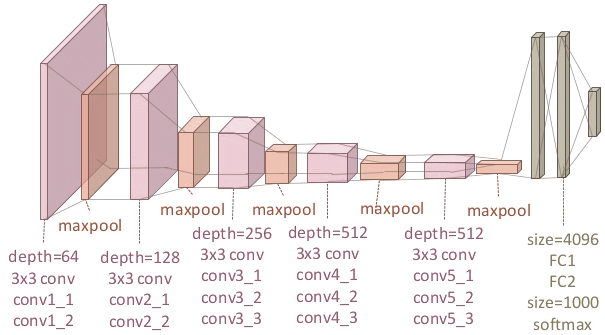
\includegraphics[width=1.0\linewidth]{vgg_architecture}
	 \caption{Arhitektura VGG-16 mreže}
 	 \label{fig:VGGArchitecture}
\end{figure}
Mana i prednost \emph{VGG-16} arhitekture je što je prostorno velika.
Oko \texttt{60MB} u svojoj cjelini sa čak \texttt{160M} parametara za treniranje što je odlična stvar za ponovno korištenje mreže za druge primjene. \\
Jedna od tih primjena je \emph{SSD} mreža, koja na svom početku sadrži baš \emph{VGG-16} arhitekturu, sve do gusto spojenih slojeva koje odbacuje.

\subsection{SSD arhitektura}
Razlog zbog kojeg \emph{SSD} mreža koristi \emph{VGG-16} kao baznu mrežu je njezina snažna performansa na slikama visoke kvalitete i popularnost gdje tehnika \emph{transfer learning}-a pomaže pri dobrim rezultatima.
Umjesto gusto spojenih slojeva \emph{SSD} mreža dodaje još konvolucijskih slojeva koji dalje izvlače značajke i progresivno smanjuju ulaz svakom dubljem sloju (\cite{liu2016ssd}).
Cijela arhitektura \emph{SSD} mreže vidljiva je na slici ~\ref{fig:SSDArchitecture}
\begin{figure}[h!]
	\centering
	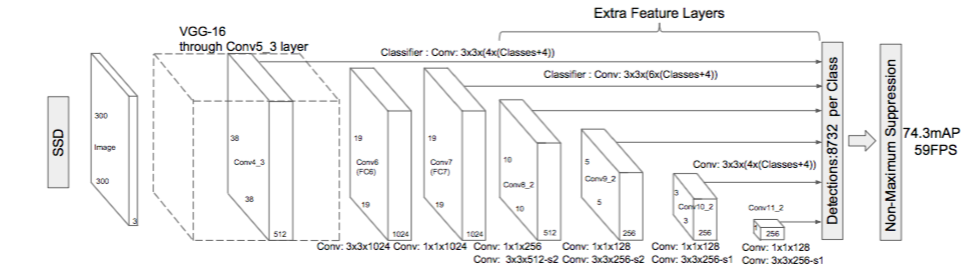
\includegraphics[width=1.0\linewidth]{ssd_architecture}
	 \caption{Arhitektura SSD mreže}
 	 \label{fig:SSDArchitecture}
\end{figure}
Slojevi dodani na baznu mrežu dodani su s ciljem da proizvedu sljedeće značajke:


\chapter{Učenje}
\section{Treniranje SSD neuronske mreže}
\subsection{Visoki pogled na treniranje}
Bitna razlika u treniranju \emph{SSD} mreže i tipične \emph{R-CNN} mreže slične zadaće je ta da "ground truth" podatak mora biti dodjeljen točnom izlazu iz fiksnog skupa izlaza detektora (\cite{liu2016ssd}).
Na sličan način radi i veliko poboljšanje na \emph{R-CNN} arhitekturu, \emph{Faster R-CNN}. \\
Kao i kod klasičnih neuronskih mreža, primjenjuje se funkcija gubitka, a za određivanja težina koristi se \emph{back propagation} od kraja do kraja.
Prije početka treniranja također se određuju pretpostavljeni kvadrati, različite skale za detekciju i strategije za povećanje podataka. \\
O pretpostavljenim kvadratima, skalama za detekciju i strategijama pisati ću u nastavku.
\subsection{Određivanje pozicije objekata}
Tijekom treninga, cilj je odrediti koji pretpostavljeni kvadrati najbolje odgovaraju "ground truth" kvadratima objekta, to jest onima specifiranim u dataset-u.
Nakon što se odrede najprecizniji kvadrati, mreža se sukladno tome dalje prilagođava.
Za svaki "ground truth" kvadrat imamo na izbor više pretpostavljenih kvadrata, različitih lokacija, skala i omjera.
Želimo naći onaj koji ima najveći \emph{jaccardov index preklapanja} (dalje \emph{IoU}) (slika ~\ref{fig:JaccardIndex}).
\begin{figure}[h!]
	\centering
	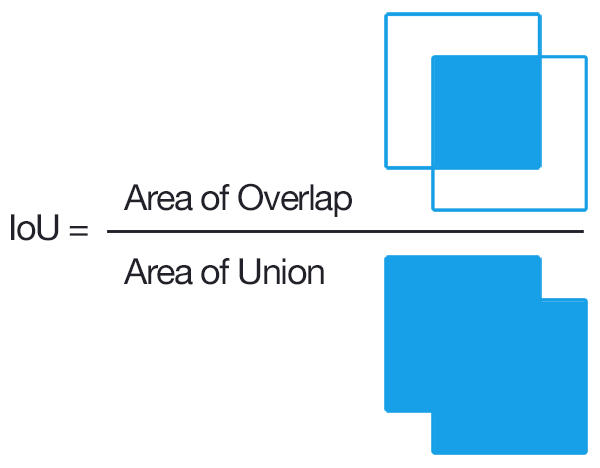
\includegraphics[width=0.6\linewidth]{iou_equation}
	 \caption{Način na koji računamo \emph{jaccardov index preklapanja, tj. IoU}}
 	 \label{fig:JaccardIndex}
\end{figure} \\
U konfiguracijskoj datoteci koja će biti priložena na kraju rada, možemo ručno odrediti od koje točke pretpostavljeni kvadrat prihvačamo.
Pretpostavljena vrijednost je da mora vrijediti $IoU \geq 0.5$.
To višestruko olakšava treniranje jer mreža zadržava više pretpostavljenih kvadrata umjesto da mora odabrati samo onaj sa najvećim preklapanjem.
\subsection{Određivanje parametara za nastavak treniranja}
Određivanje parametara bilo bi puno lakše kada bismo imali samo jedan objekt za klasificirati, no postaje kompliciranije sa više objekata.
Uzmimo $x^p_{ij}=\{1,0\}$ kao indikator za podudaranje $i$-tog pretpostavljenog kvadrata na $j$-ti "ground truth" kvadrat kategorije $p$.
Koristeći spomenutu strategiju određivanja pozicije objekata može nam se dogoditi situacija $\sum_i{x_{ij}^p} \geq 1$. \\
Ukupna funkcija gubitka računa se kao otežana suma lokalizacijskog (\emph{loc}) i klasifikacijskog (\emph{conf}) gubitka:
$$L(x,c,l,g)=\frac{1}{N}(L_{conf}(x,c)+\alpha L_{loc}(x,l,g))$$
$N$ nam predstavlja broj "pogođenih" pretpostavljenih kvadrata. Naravno, ako je $N=0$, postavimo da je gubitak također $=0$.
\subsubsection{Lokalizacijski gubitak (\emph{loc})}
Za izračun lokalizacijskog gubitka koristimo \emph{Smooth L1} između predviđenih i "ground truth" kvadrata.
$$L_{loc}(x,l,g)=\sum_{i\in Pos\ m \in\ (cx, cy, w, h)}^{N} \ \sum x_{ij}^k\ smooth_{L1}(l_i^m - \hat g_j^m)$$
\subsubsection{Klasifikacijski gubitak (\emph{conf})}
Klasifikacijski gubitak računa se kao \emph{softmax} svih klasa koje podržavamo. 
$$L_{conf}(x,c)=-\sum_{i \in Pos}^N x_{ij}^p \log(\hat c_i^0) - \sum_{i \in Neg} \log(\hat c_i^0 ) \ {gdje} \ \hat c_i^p=\frac{\exp(c_i^p)}{\sum_p \exp(c_i^p)}$$


\chapter{Rezultati}
\section{Opis rezultata}
Mreža se s vremenom ponašala iznimno zanimljivo.
Već u prvih par koraka vrijednost ukupne funkcije gubitka ~\ref{eq:lokKlasLoss} brzo se spustila sa $\geq 50$ na $\leq 10$.
No nevjerojatno dugo joj je trebalo da se spusti na vrijednost $\leq 4$.
Razlog tome je pretpostavljam određeni broj \emph{false positive}-a (Slika ~\ref{fig:FalsePositive}) unutar skupa podataka.
Naime, \emph{false positive} slike nastale su primjenom transformacija nasumično generiranim parametrima koji su se našli na rubu prihvatljivih vrijednosti.
Nažalost, zbog velikog broja slika (nakon svih generiranja, pokušaja i učenja $\geq 20000$) nisam ručno mogao izbaciti sve.
Ipak, smatram da je određeni mali broj takvih slika neophodan za uspješno učenje slike. \\
Nakon ukupno $500 000$ koraka, tj. $80$ epoha po formuli ~\ref{eq:stepEpoch},  ukupni gubitak iznosio je $3.879$ gdje je po izgledu dosegao asimptotu.
\section{Prikaz rezultata}
Na slici ~\ref{fig:IndividualDigit} prikazana je prva uspješno detektirana i klasificirana slika, dotad ne viđena mreži.
Postotak pouzdanosti ($0.54$) je jasno na donjoj granici i naslućuje prve uspjehe prilagođenoj neuronskoj mreži koja nikad prije nije bila osmišljena za detekciju teksta.
\begin{figure}
	\subfloat[\emph{False positive} slika koja sadrži neodređeni element naizgled nevidljiv zbog nepravilnih transformacija primjenjenih na istom] {%
		
\includegraphics[width=0.45\linewidth]{false_positive} %
		\label{fig:FalsePositive}
	}
	\qquad
	\subfloat[Prva detekcija računalno generirane  znamenke 3 na slici uz mali postotak pouzdanosti] {%
		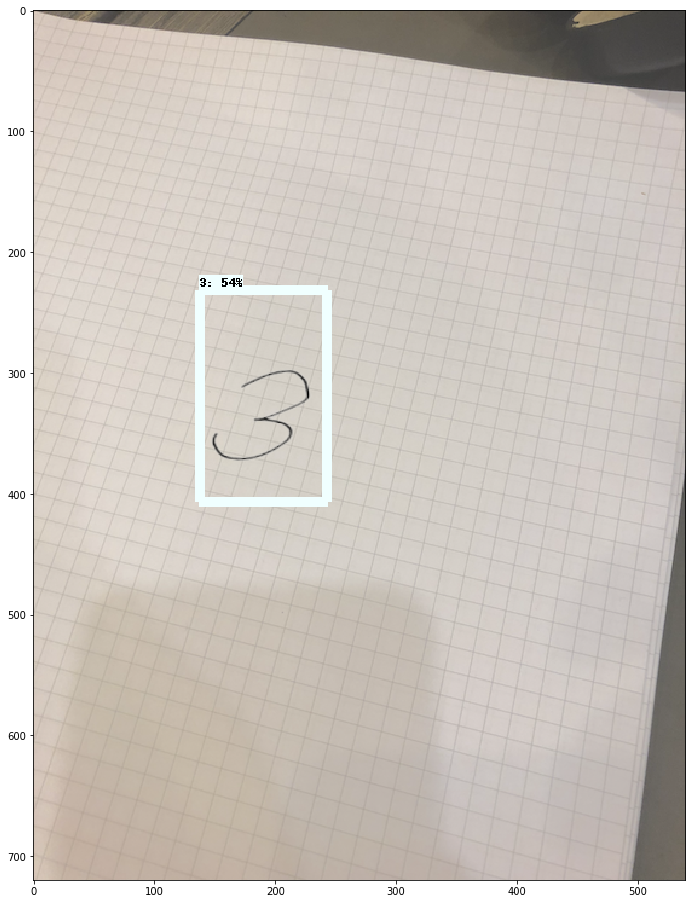
\includegraphics[width=0.45\linewidth]{three} %
		\label{fig:IndividualDigit}
	}
\end{figure} \\
S vremenom, mreža je postajala sve pouzdanija te je nakon $\approx 350000$ koraka prvi puta prepoznala cijeli izraz, odnosno sve članove istog.
Priložene slike (~\ref{fig:ExpressionA} i ~\ref{fig:ExpressionB}) također nikad prije nisu bile viđene od mreže i dobar su primjer jer se jasno vidi kako, iako su slike identične, nakon određenog dodatnog broja koraka mreža preciznije određuje granice individualnih simbola i puno pouzdanije prenosi koji su. \\
\begin{figure}
	\subfloat[Pouzdanost i preciznost nakon $350000$ koraka] {%
		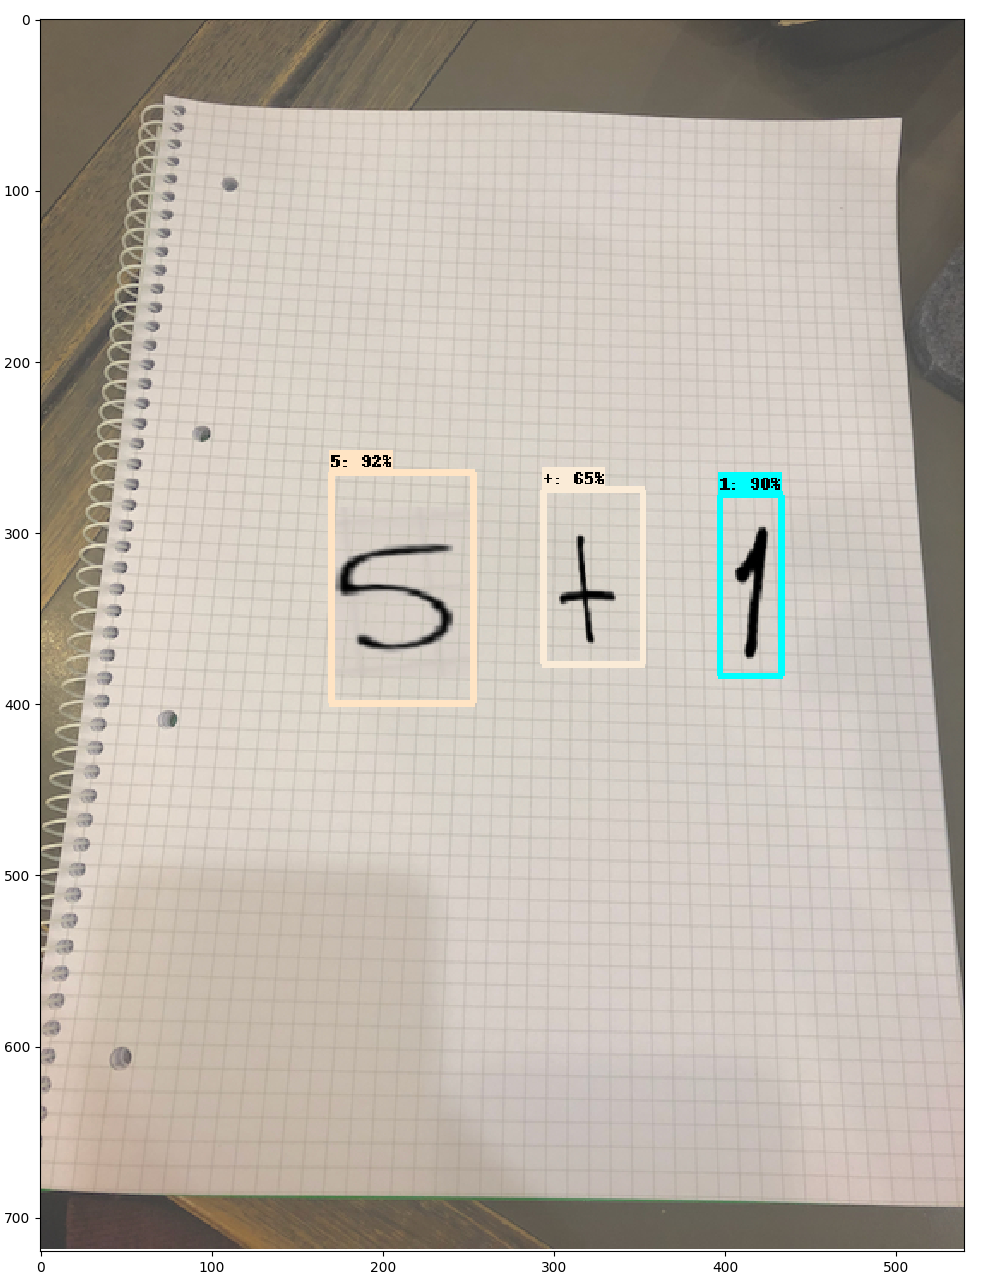
\includegraphics[width=0.45\linewidth]{first_generated_eqn} %
		\label{fig:ExpressionA}
	}
	\qquad
	\subfloat[Pouzdanost i preciznost nakon $500000$ koraka] {%
		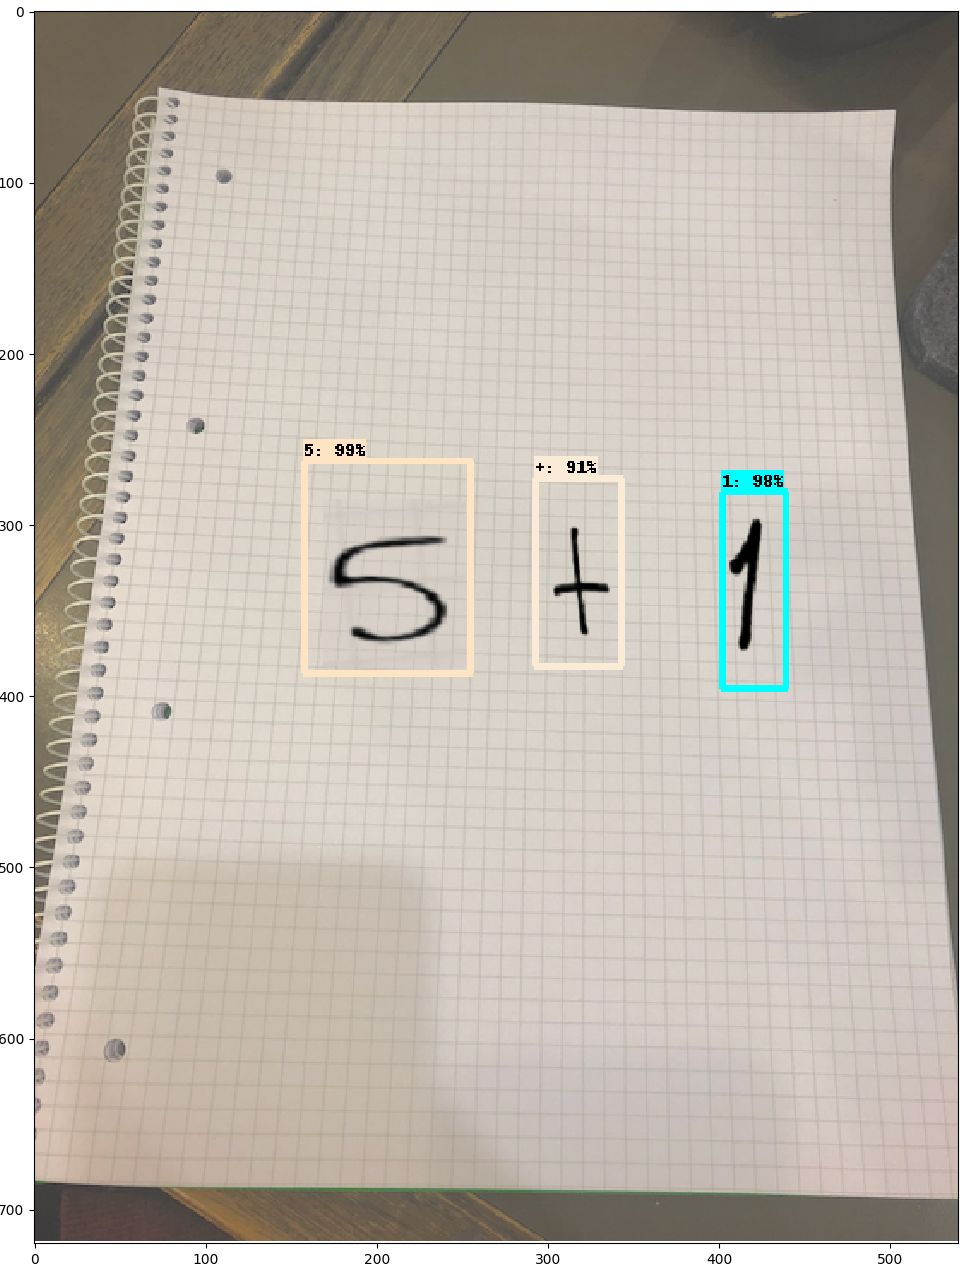
\includegraphics[width=0.45\linewidth]{last_generated_eqn} %
		\label{fig:ExpressionB}
	}
\end{figure} \\
Nakon završenog učenja bilo je zanimljivo probati je li mreža ušla u fazu \emph{prenaučenosti}-a što se vrlo lako moglo provjeriti dajući joj stvarni, rukom napisani primjer kojeg je bez problema detektirala i klasificirala (Slika ~\ref{fig:Handwritten}).
\begin{figure}[h!]
	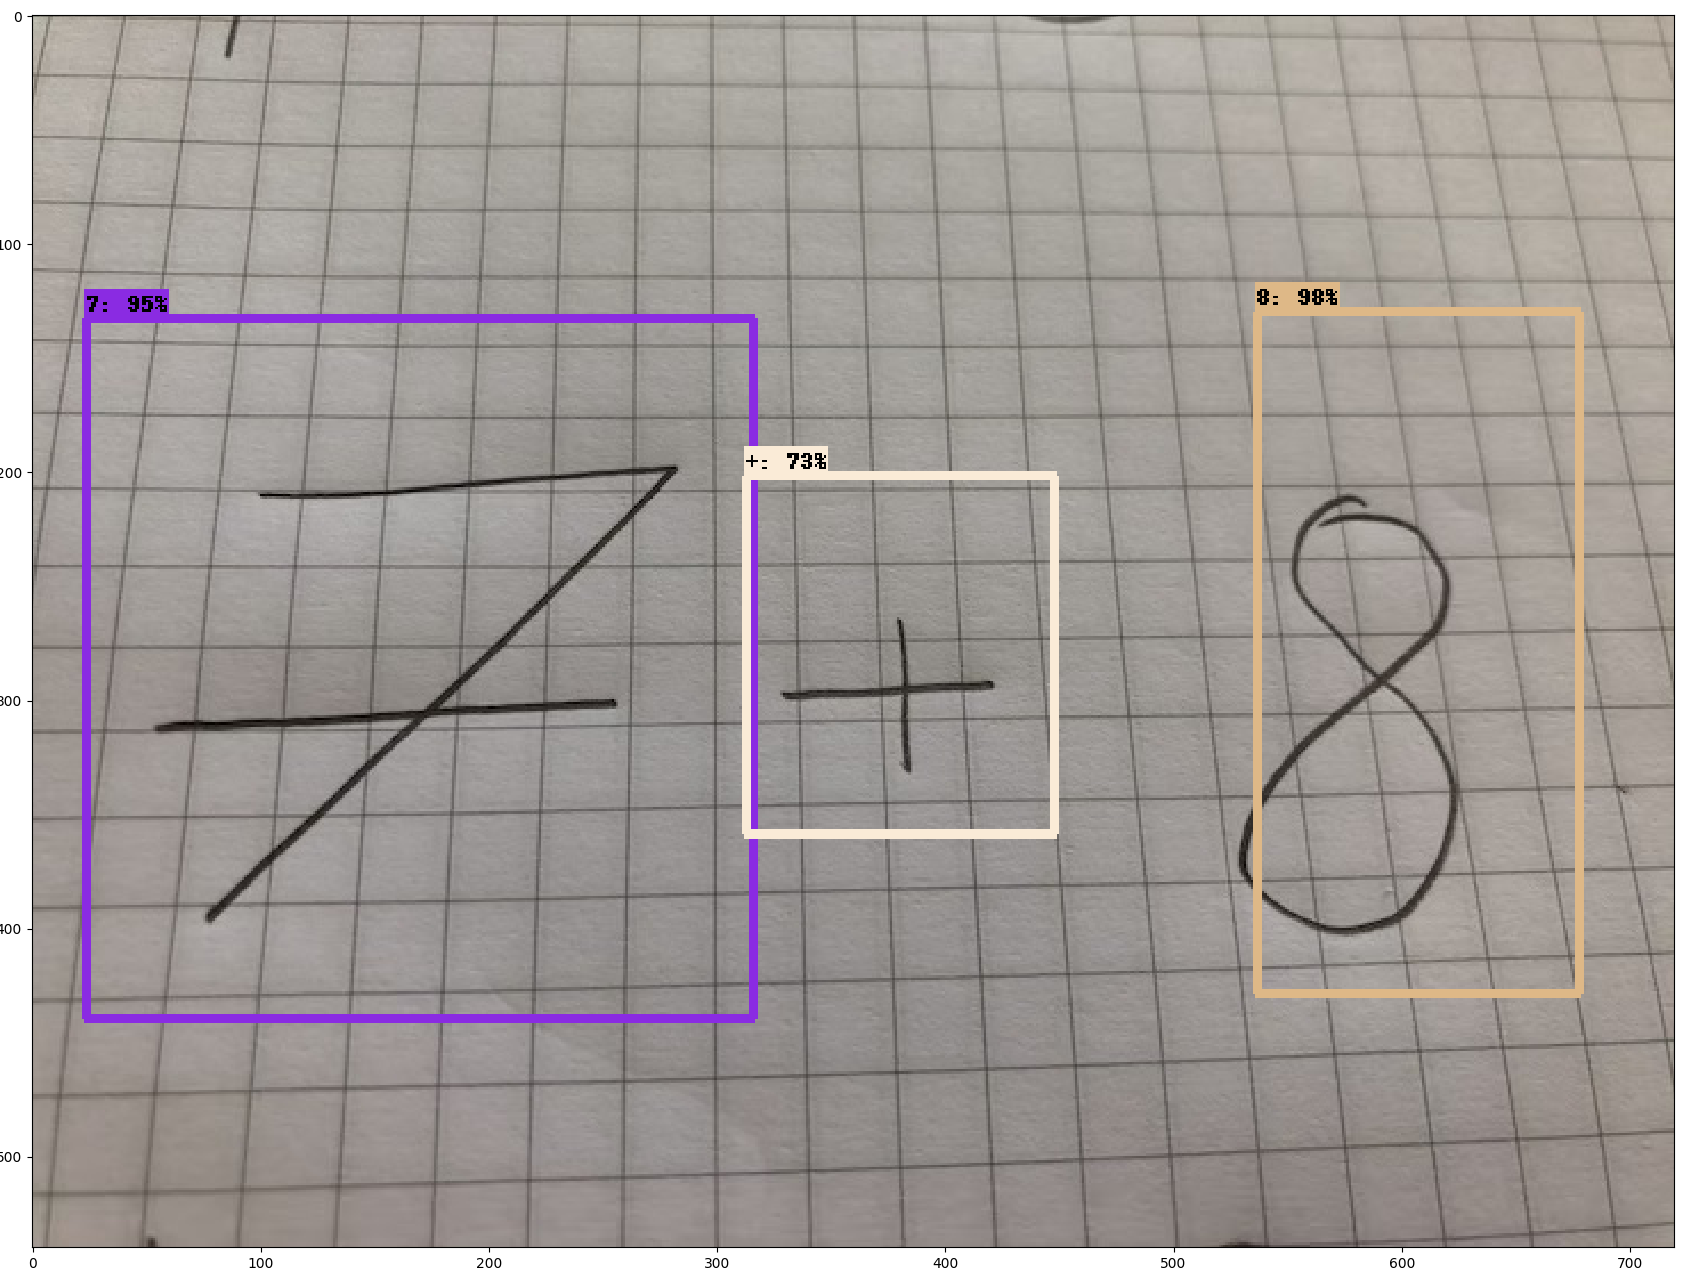
\includegraphics[width=0.5\linewidth]{handwritten}
	\caption{Jednostavan ručno napisan matematički izraz koji prikazuje uspjeh rada mreže na istom}
	\label{fig:Handwritten}
\end{figure}
\section{\emph{Tensorboard} rezultati}
Velika prednost korištenja \emph{Tensorflow}-a nad ostalim knjižnicama za duboko učenje je korištenje \emph{Tensorboard}-a koji fantastično i uživo prikazuje napredak učenja mreže zadanog zadatka.
Slika ~\ref{fig:losses} prikazuje način na koji \emph{Tensorboard} prikazuje gubitke kroz vrijeme, dok ~\ref{fig:totalLoss} prikazuje ukupan gubitak kroz vrijeme.
Naravno, naprednim korištenjem alata mogu se prikazati i ostale korisne stvari kao što je prikaz rada mreže na određenom broju slika uživo, no za moje potrebe, prikaz gubitka je bio dostatan za razumjevanje procesa učenja.
\begin{figure}
	\subfloat[Napredak dvije komponente gubitka kroz vrijeme] {%
		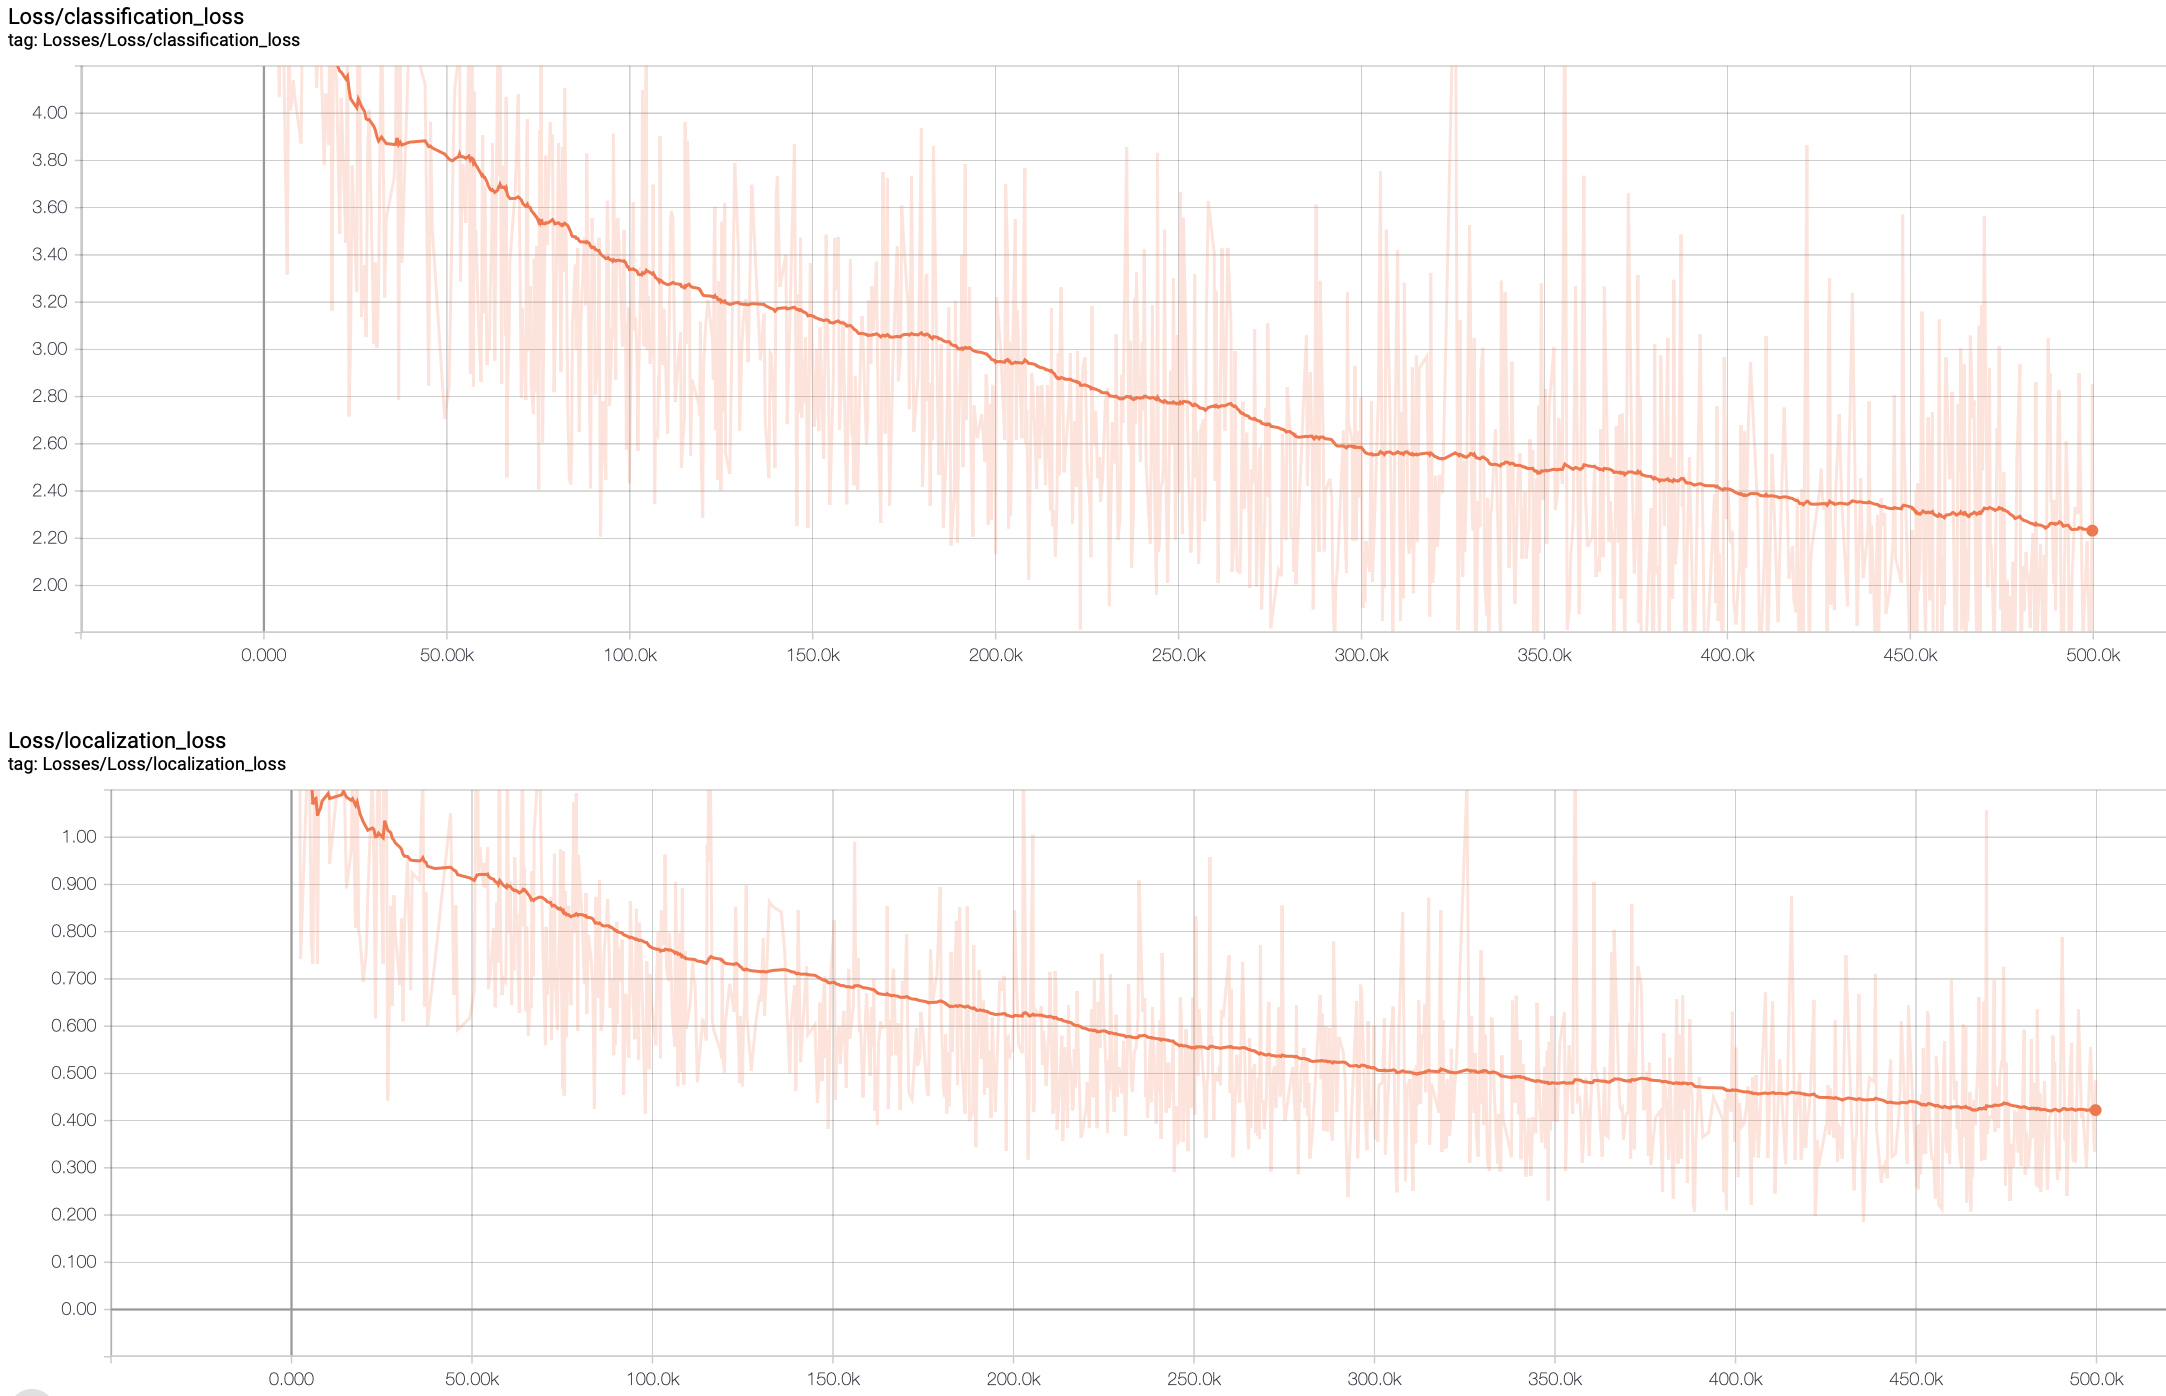
\includegraphics[width=1.0\linewidth]{losses} %
		\label{fig:losses}
	} \\
	\subfloat[Ukupan gubitak nastao od lokalizacijskog i klasifikacijskog gubitka kroz vrijeme] {%
		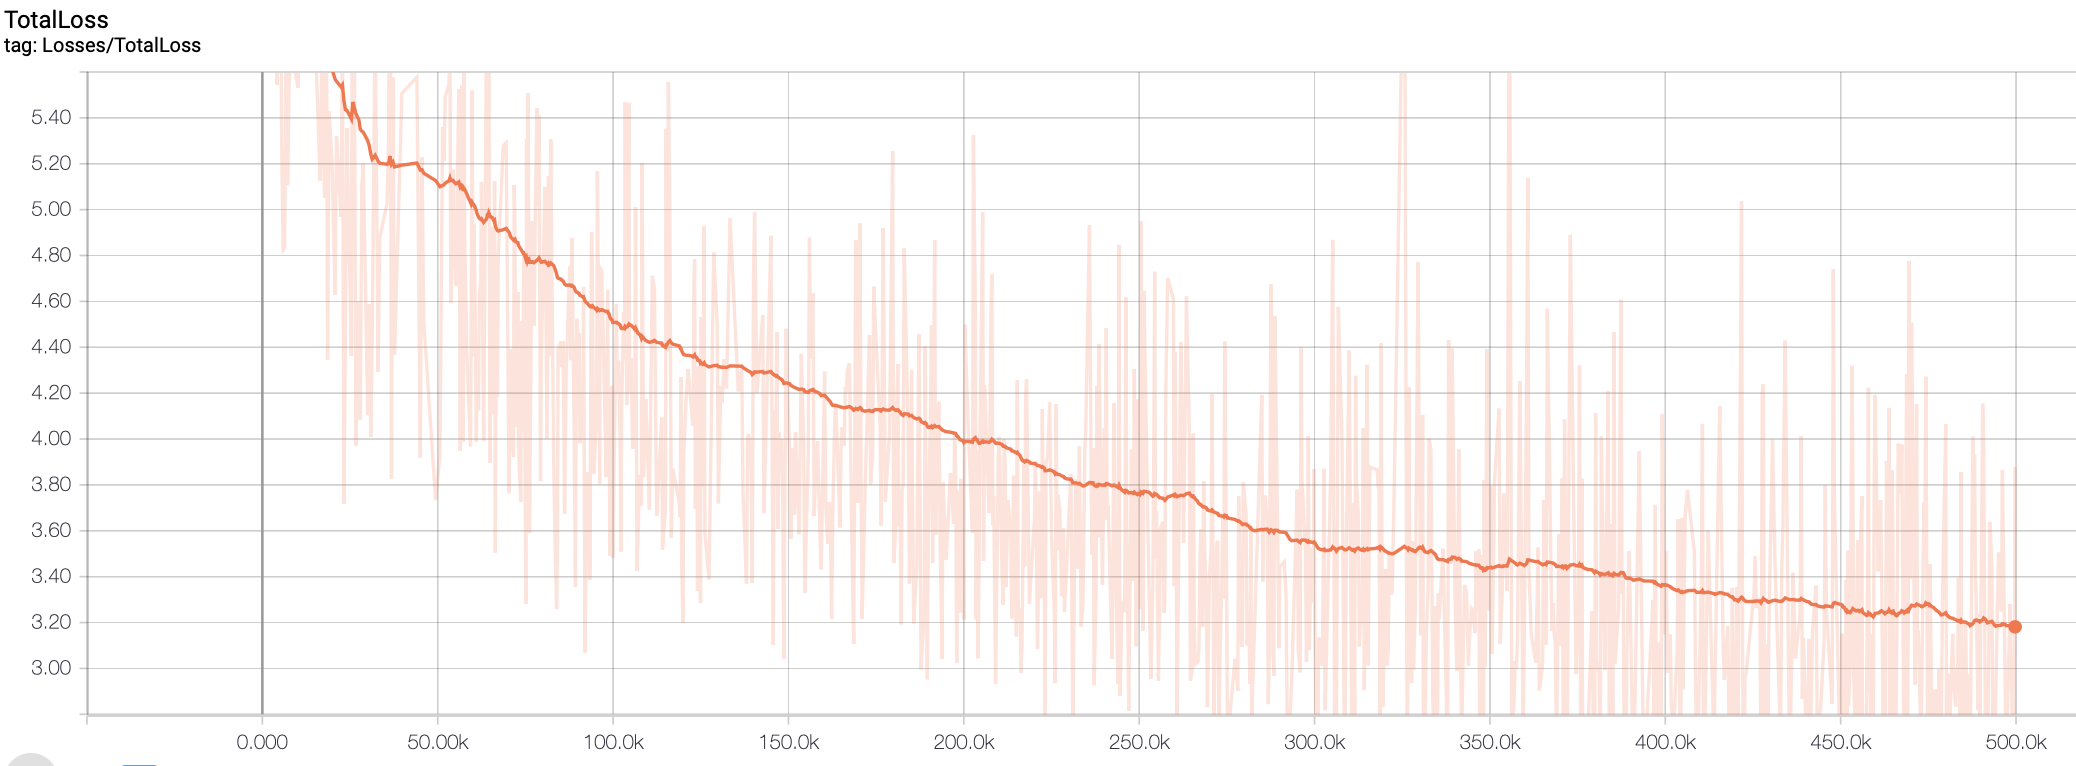
\includegraphics[width=1.0\linewidth]{total_loss} %
		\label{fig:totalLoss}
	}
\end{figure}


\chapter{Programska podrška}
\section{Korištenje programske podrške}
Programska podrška napravljena u svrhu demonstracije svih spomenutih značajki ima dva glavna načina rada.
Ispis pronađenog teksta i pretraga unešenog teksta.
\subsection{Ispis pronađenog teksta}
Način rada koji se pretpostavlja da korisnik želi koristiti.
Kroz argument predaje se apsolutna putanja do slike nad kojom se želi izvršiti detekcija a program na standardni izlaz ispisuje pronađeni tekst.
Pronađeni tekst zatim prolazi evaluaciju koja je dio standardne biblioteke programskog jezika \emph{Python}.
Ako je izraz moguće evaluirati npr. "$2 + 2$", na standardni izlaz ispisuje se rezultat operacije kao što je vidljivo na slici ~\ref{fig:output}.
\begin{figure}[h!]
	\centering
	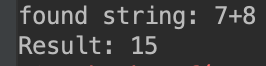
\includegraphics[width=0.6\linewidth]{CommandLineOutput}
	 \caption{Izlaz nakon evaluacije pronađenog teksta}
 	 \label{fig:output}
\end{figure}
\subsection{Pretraga unešenog teksta}
Drugi način rada nakon što slika prođe kroz korak detekcije i klasifikacije teksta sprema pronađeni izraz u obliku niza.
Korisnik pri izvršavanju programa prethodno mora unjeti regularni izraz koji opisuje ono što želi znati nalazi li se na slici na što program odgovara na standardni izlaz postoji li ili ne.
Način pretrage unešenog teksta dostupan je postavljanjem zastavice \texttt{r} kao argument pri pokretanju.
\section{Budući rad}
Iako programska podrška trenutno pruža osnovnu funkcionalnost, postoji dosta prostora za rast i napredak.
Trebala bi se znati vršiti segmentacija izraza po retcima jer se trenutno pronađeni objekti sortiraju s lijeva na desno i na isti način evaluiraju.
Segmentacija po retcima pružila bi mogućnost za kompliciranije izraze i kompletniju implementaciju. \\
Također, bilo bi korisno mrežu spojiti sa jednostavnim grafičkim sučeljem koje bi znatno olakšalo korištenje van komandne linije.


\chapter{Zaključak}
Ovaj rad obuhvatio je cjelokupni cjevovod jednog ciklusa pripreme duboke neuronske mreže za specifičan zadatak.
Proces stvaranja slika omogućio je gotovo neograničen skup podataka za neuronsku mrežu.
Isti skup podataka korišten je za za prenamjenjivanje \emph{SSD} neuronske mreže za detekciju na zadatak prepoznavanja rukom napisanih simbola.
U detalje je opisana arhitektura spomenute mreže i metode koje koristi za računanje kvalitete izlaza.

Inicijalno, mreža je bila naučena za prepoznavanje objekata unutar $6000$ kategorija.
Dalje je korištena metoda prenamjenjivanja mreže na druge kategorije koristeći postojeće težine.
Spomenuta pretpostavka uvelike je olakšala i ubrzala cijeli postupak jer mnogi primitivi koji postoje unutar tih $6000$ kategorija, pojavljuju se i u simbolima.

Nakon procesa učenja u $15 000$ koraka tj. $80$ epoha, dosegnuta je zadovoljavajuća točka preciznosti i pouzdanosti na večini simbola.
Jedini simbol, koji nije uspješno naučen je simbol množenja što je i jedan od budućih izazova.
Ostvariti zadovoljavajuću preciznost na svim simbolima i vršiti segmentaciju po retcima.
Također, preporučuje se i korištenje drugih arhitektura (npr. \emph{Faster R-CNN}) te usporedba rezultata.
 


\bibliographystyle{ieeetr}
\bibliography{literatura}

\begin{sazetak}
Rad je opisao postupak automatskog pozicioniranja, transformiranja i spremanja tekstovnih elemenata na sliku u oblik čitljiv neuronskoj mreži.
Korišten je \emph{Tensorflow Object Detection API} za postupak učenja detekcije i klasifikacije istih elemenata na slici.
Ako je na slici pronađen matematički izraz, evaluacijom je dan rezultat istog.

\kljucnerijeci{detekcija, klasifikacija, duboke neuronske mreže, strojno učenje, Tensorflow, Keras, generiranje slike}
\end{sazetak}

\engtitle{Detection and classification of text based elements on an image using deep neural networks}
\begin{abstract}
This paper describes the whole process of automatically positioning, transforming and saving textual elements on an image in a form that is readable by a neural network.
\emph{Tensorflow Object Detection API} is used for training detection and classification of generated elements on an image.
If an image contains a mathematical expression, evaluating returns the solution.

\keywords{detection, classification, deep neural networks, machine learning, Tensorflow, Keras, generating images}
\end{abstract}

\end{document}
